\chapter{Introduction}\label{ch:introduction}

\section{Objectives of the report}\noindent
This work concerns the use of dynamic optimization - optimal control and calculus of variations - techniques to address the problem of optimally controlling an Unmanned Aircraft Vehicle (UAV) in an uncertain environment. Special emphasis will be placed in avoiding collision with obstacles.

Modern day avoidance systems are based on rule system implementation \cite{benjamin2006navigation}. Rule systems are technical bridge between law and implementation. These rules are putting additional high level constraints to optimal control problem.  Rich constraint programming languages have been developed for expressing and combining constraints and specifying search procedures at a high level of abstraction. Local search approaches to combinatorial optimization are able to deliver optimal control to vehicles \cite{hentenryck2009constraint}. The first of approaches delivered in constrained search are given \cite{grefenstette1986optimization}. All mentioned approaches revolves around keeping optimum principle in high level control in partially known environment. Methods varies from logical programming applications to performance based search. Software engineering methods for abstract path searching can be response for optimal path problem \cite{korf1985depth}.

Solution to given abstract problem consist of interdisciplinary usage of various method:
\begin{enumerate}
    \item\textit{Rule engine application} - rules impact decision making of overall system, this part of control system is viewed as event based control.
    \item\textit{Path switching} - events given by rules can impact path switching, previously optimal path may not be viable, therefore new optimal path needs to be derived in near real-time conditions. Decision making can be viewed as part of artificial intelligence field. 
    \item\textit{Higher level optimality principle} - higher level of control mechanism is used to abstract from controlled plant and enables fast optimal path calculation
    \item\textit{Lower level optimality principle}- standard low level control mechanism guarantying optimal execution of higher level control commands.
\end{enumerate}

\newpage
\section{Motivation}\noindent
Problem of obstacle avoidance can be applied to any type if vehicle \textit{ground, aerial or marine}. Obstacle avoidance can be separated into two categories. \textit{Three dimensional avoidance} for aerial and subsurface marine vehicles  and \textit{Two dimensional avoidance} for ground and surface marine vehicles. This work focus on \textit{Three dimensional avoidance} with partially known boundaries. Results of this work can be applied to both categories of \textit{subsurface marine} and \textit{aerial} vehicles. The only difference is that in \textit{subsurface marine} obstacle avoidance boundary of water surface exists. Boundary of \textit{water floor} and \textit{ground bed} are similar, despite fact that vehicles dynamics is different. Example of marine vehicle obstacle avoidance can be found in \cite{benjamin2006navigation}. Example of vehicle avoidance equipment can be found in \cite{chey1986vehicle}. There exists representations where Sonar and LiDAR Inputs are exchangeable \cite{fiorini1998motion}. 
\noindent
Optimal path planning in partially known environment is critical for following reasons:
\begin{enumerate}
    \item \textit{Safety guarantee} - guarantee safety of vehicle and prevent it destruction.
    \item \textit{Energy consumption} - prolong vehicle operational capabilities to maximal extent.
\end{enumerate}
Main motivation is  \textit{energy consumption aspect}. Path planning for UAV with focus on low energy consumption is given by \cite{bortoff2000path}. Some of the works are taking inspiration form  nature, like \cite{ma2007improved}. Other was specialized on predictive control in urban environment \cite{singh2001trajectory}. Proposition for optimal control problem to optimal parameter problem is given by \cite{hull1997conversion}. This proposition is key enabler for conversion of optimal control problem in continuous time to discrete parameter problem. 
\noindent
The problem of many optimal control approaches mentioned beforehead is that they are using optimum principle in continuous time. This work focus on The proposed approach combines abstract sensing technology with techniques based on controlled invariance in discrete time. Sensors fusion provides a abstract representation of the world in the field of view of the sensors. Controlled invariance techniques provide a characterization of flight envelopes that by design avoid obstacles under reasonable assumptions. 
\begin{figure}[H]
    \centering
    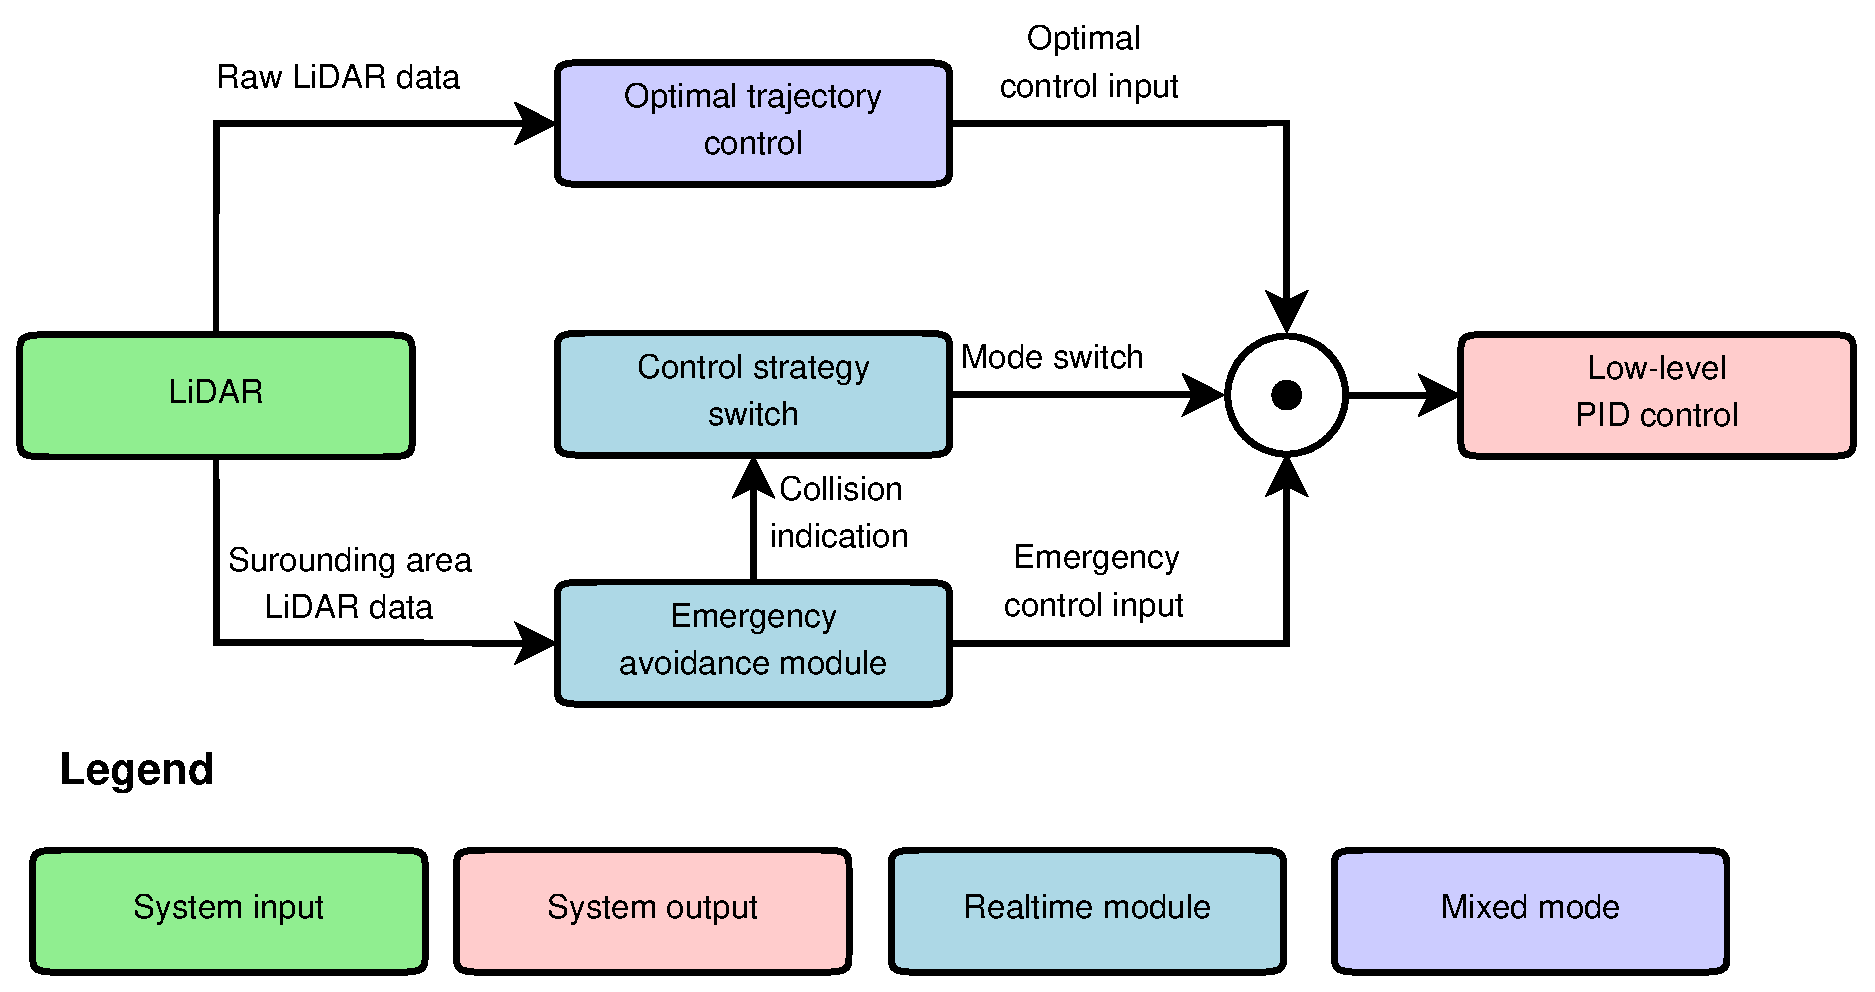
\includegraphics[width=10cm]{Pics/35_ControlConcept.eps}
    \caption{Control concept scheme}
    \label{fig:ControlConcept}
\end{figure}
\noindent
The approach presents a nested solution to control design depicted in Figure \ref{fig:ControlConcept}. There is a nominal trajectory for the UAV that may be generated by an  \textit{Optimal trajectory control} module. Sensor will continuously scan the environment for obstacles. If an obstacle crosses a pre-computed safety zone then an \textit{Emergency avoidance module} is invoked to override the trajectory tracking controller. \textit{Emergency avoidance module} is invoked and keeps vehicle at semi-optimal avoidance path, with premise that vehicle will return to original planned path. The safety zone is computed using invariance techniques based on reach set computations. When the obstacle no longer presents a threat (i.e., it does not belong to the safety zone) control is returned to \textit{Optimal trajectory control} module. This nested control approach entails  a \textit{Control strategy switch} will override control input of system and starts avoidance maneuver to achieve \textit{reactive avoidance}.
%\textit{UAV} is usually used for two types of missions, or rather \textit{operation types}:
%\begin{enumerate}
%    \item \textit{Delivery} - deliver usable point from point A to point B.
%    \item \textit{Surveillance} - fly trough defined area. 
%\end{enumerate}
%It is expected that UAV returns from mission unharmed. 
%\section{Approach}



\section{Goals}\noindent
Main goals of this work is to provide following artefacts, which will contribute to complex obstacle avoidance system:
\begin{enumerate}
    \item\textit{Optimal control translation from higher to lower level} - translation of high level commands to lower level continious signal. This is one of main goal of the thesis
    \item\textit{Control architecture for optimal control} - provide control framework architecture combining event based, discrete time higher level optimal control and continuous lower level optimal control.
    \item\textit{Decision frame for high level decisions} - outline decision frame for event based system in control switch (fig. \ref{fig:ControlConcept}).
\end{enumerate}
%\noindent
%The goal of the research is to develop an integrated approach to real-time obstacle detection and avoidance for Unmanned Air Vehicles (UAV) based on %\textit{LiDAR} technology. The approach concerns the solution of the following sub-problems:
%\begin{enumerate}
%    \item \textit{Obstacle detection and sensor fusion} - processing \textit{LiDAR} data into an unified and compact data representation for obstacle detection. 
%		
%    \item \textit{Real-time reactive obstacle avoidance} - identify safety problems and perform avoidance maneuvers with safety guarantees when collisions are possible and return control to nominal controller when collision is avoided.
%\end{enumerate}

\section{Organization of the report}\noindent
Report is organized in following manner:
\begin{itemize}
    \item\textit{Chapter \ref{ch:introduction}.} presents motivation, goals and objectives of report.
    \item\textit{Chapter \ref{ch:UAVControlProblem}.} defines control principle with emphasis to principle of optimality. It also outlines assumptions used for proof of concept.
    \item\textit{Chapter \ref{ch:stateofArt}.} provides overview of reach sets, movement automaton and other theoretical supplements used in this work.
    \item\textit{Chapter \ref{ch:problemFormulation3D}} provides problem formulation and it is addressing issues of optimal control.
    \item\textit{Chapter \ref{ch:controlapproach3D}} describes control approach in detail with used techniques with emphasis on optimal control.
    \item\textit{Chapter \ref{ch:controlapproach3D}.} revolves around control approach on higher level framework and movement automaton $\mathscr{MA}$ movements $\mathscr{m_i(t_i)}$ translation to continious signal.
    \item\textit{Chapter \ref{ch:simulationResults}.} is focused on simulation results of proposed optimal control approach, it outlines preliminaries of obstacle avoidance framework.
\end{itemize}


 





